\subsection{Detecting Misuse of Compute Resources} \label{sec:sensor-passwordcrack}

\begin{figure}[tb]
\centering
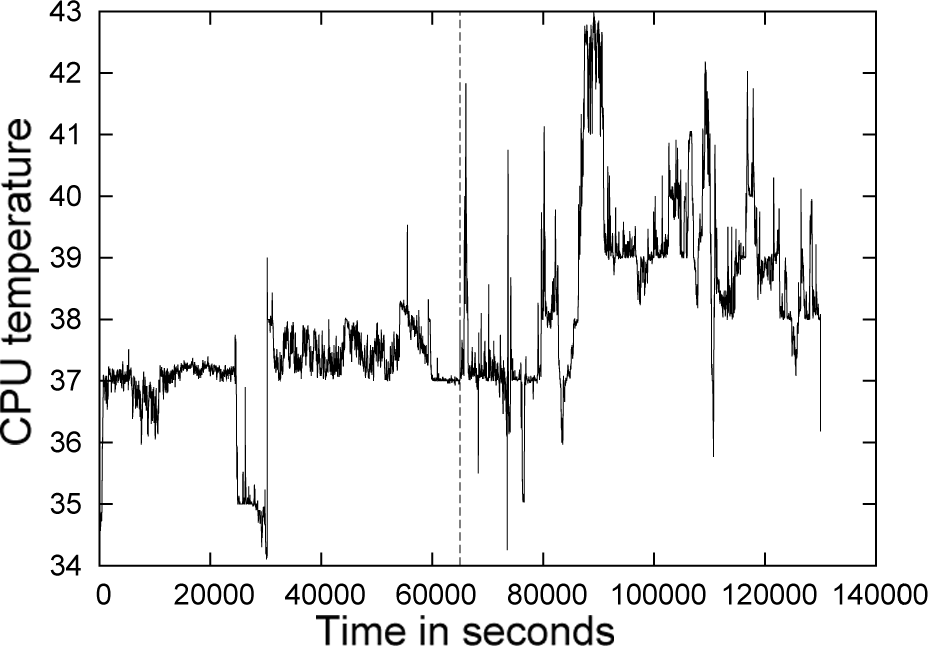
\includegraphics[width=0.5\textwidth]{sensor/normal-cat.png}
\caption{CPU temperature variation when user is absent and present. 
The user is absent from 0 to 64,000 second;
and present from 64,000 second onwards. The user is absent left of
the vertical dotted line and present to the right of the line.
} 
\label{fig:temp-norm}
\end{figure}


\begin{figure}[tb]
\centering
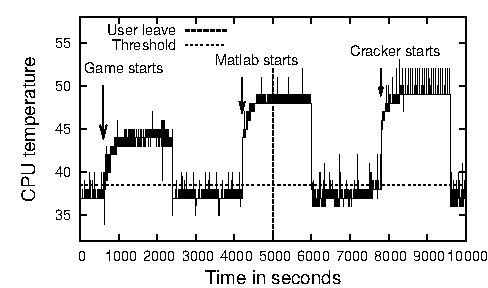
\includegraphics[width=0.6\textwidth]{sensor/temp-activities.pdf}
\caption{CPU temperature variation during various activities.}
\label{fig:temp-activities}
\end{figure}

Bots are often recruited to invert cryptographic functions to break
passwords. Inverting such functions requires extensive computations
which are distributed to the bots. To detect such activities, we
look for increases in the CPU load when the user has been absent for a
while. As CPU load is internal to the host,
we rely on CPU temperature as an indirect measurement which can
be obtained by an external sensor.

Figure~\ref{fig:temp-cpuload} shows the correlation between CPU load
and temperature.
The correlation is good but we can see that there is
noise and other fluctuations in the measurement.
Thus, this is an example of a sensor measurement which is imperfect and
has noise.
Figure~\ref{fig:temp-norm} shows the temperature when a user
is present and absent. Note when the user is absent, the temperature
is around 37$^\circ$C, with less variability.  We measured the
temperature during automated software update and found the
temperature increase of 2-3$^\circ$C.

When we employ CuSum to detect the increase in CPU temperature,
we can determine the thresholds $a$,
$N$ and $t$ from CPU temperatures in normal usage.
Figure~\ref{fig:temp-norm} shows normal temperature variations during user
presence and absence. From the observation of Figure~\ref{fig:temp-norm},
we set the upper bound of system idle
temperature to be $a=38.5^\circ$C. We set the threshold for
the accumulated increase in temperature as $N=2400$ in 30 minutes.
This threshold $N$ is chosen to allow software update that increases
the CPU temperature by 2$^\circ$C and lasts for 20 minutes.\footnote{
Windows Update may run when the user is absent.
}
We set a grace period of $g=10$ minutes at the transition
from user presence to absence, that is, if the changepoint is
detected within 10 minutes after a user leaves, the alarm is not
activated.\footnote{
The grace period is a window for the bot to perform its computation but
it is only a small fraction of the time available to the bot, so it still
significantly limits the amount of computation which can be performed.
}
For comparison, the thresholds of CPU temperature for rate based detection is set as $T_r = a + N/t = 39.83^\circ$C, and the threshold for moving average detection is $T_m = 40^\circ$C. We note that the instantly measured CPU temperature that our sensor outputs has granularity of degrees.

\begin{table}[tb]
\centering
\begin{tabular}{|c|c|c|c|}
\hline
Detection & Rate & Moving & Changepoint \\
Algorithm & (sec) & Average (min) & (min) \\
\hline
Game            & 14 & 11  & 10.4   \\
\hline
Matlab           & 4 & 8.5 & 5.2   \\
\hline
Password Cracker & 2 & 7.1 & 4.5   \\ [0.5ex]
\hline
\end{tabular}
\caption{Detection time of CPU intensive activities,
using rate based detection, moving average detection,
and changepoint detection (The upper bound of normal CPU temperature
is $a=38.5^\circ$C,
and the detection threshold $N=2400$ in $t=30$ mins).}
\label{tbl:detect-CPU}
\end{table}

Figure~\ref{fig:temp-activities} shows the temperature during various
computation tasks.
Table~\ref{tbl:detect-CPU} shows the detection time of computation
intensive activities, using different detection methods.
Rate based detection detects the computation activities in seconds;
moving average takes 7 to 11 minutes;
while changepoint detection has a detection time that is in between.
The changepoints in temperature for playing games
and running Matlab are detected 10.4 minutes and 5.2
minutes respectively after they start. Since the user is present or
has just left when the changepoint occurs, the activities are considered
initiated by the user and accepted as normal. The password cracker
activity triggers an alarm 4.5 minutes after it starts. Since the
changepoint is detected when user is absent, it is considered as
malicious computation. If the malicious computation executes during
user presence, it can be noted by the user since there could be an
overall system slowdown.

\begin{figure*}[tb]
\centering
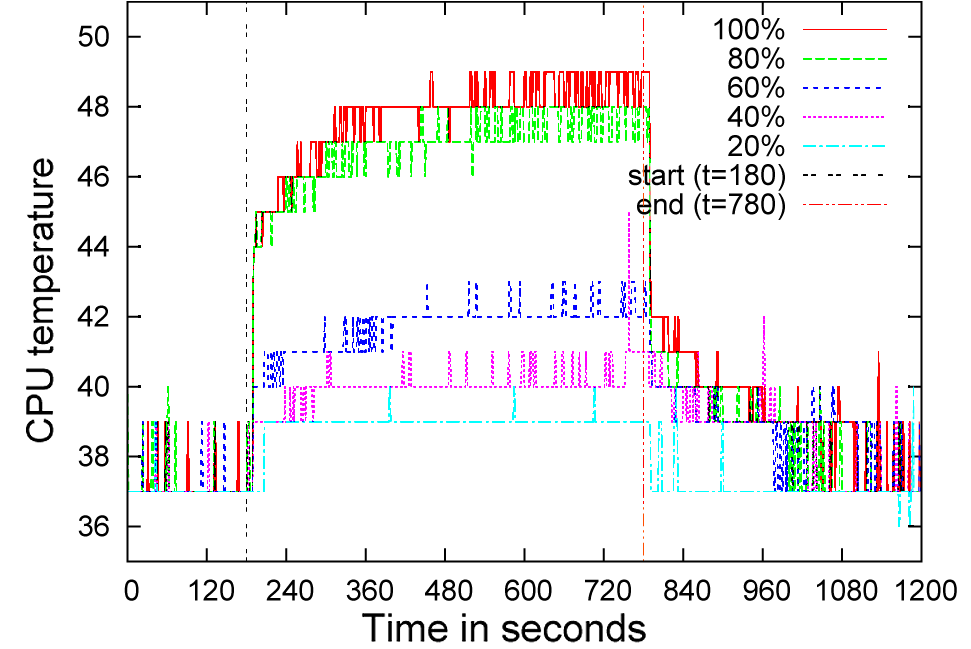
\includegraphics[width=0.6\textwidth]{sensor/passwd-line.png}
\caption{Correlating attack intensity and CPU temperature. }
\label{fig:pwd-vary}
\end{figure*}

Although rate based detection is very quick, it is highly sensitive to
false positives and negatives. When the computation intensive programs start, 
this clearly causes a substantial increase in CPU workload
which leads to a sudden increase in CPU temperature. 
Hence, rate based detection is quick in detecting CPU activity.
However, very often, non-compute intensive programs can temporarily raise
the CPU temperatures by $2^\circ$C upon process startup and return to normal
after that. This will cause false positive for a rate based detector. 
On the contrary, a moving average detector will treat
sudden changes of CPU temperature as a gradual transition 
of the average temperature. Thus, the amount of time
it takes to detect can vary significantly,
depending heavily on the initial states. 
Detection using changepoint is usually more efficient than moving average, 
and is more reliable than rate based detection.

%After the program initialization which causes a temporary and sudden increase of the CPU temperature, the CPU temperature lowers before it climbs up again and 
%remains high. Changepoint monitors the conditionally accumulated excess of CPU temperature.
%
%To reduce potential false positives, the detection threshold for rate based detection would necessarily be much higher.

We also conducted an experiment which varies the intensity of the
CPU usage. This investigates if the CPU usage can be detected when
the malware throttles its computation at a lower rate. CPU usage is
controlled as follows: for each one-second interval, the bot
computes at full speed for $x$ seconds and then sleep for $1-x$
seconds, where $x<1$. We denote the CPU usage to be $100x$\% in
Figure~\ref{fig:pwd-vary}. We carry out the attack for 600 seconds (starts
at 180 seconds and ends at 780 seconds).
Note that after the attacks
stop, the temperature gradually returns to normal.  For the password
computation running at 100\% usage, we detect the change after about
4.5 minutes.  For the computation at 20\% usage, we can also detect
the change using changepoint detection, if the computation lasts for more than 20 minutes. To
evade detection, the malicious computation can only further reduce
its CPU usage or shorten its execution time.
Thus, our system effectively limits the amount of malicious computation. In contrast, at 20\% CPU usage, 
rate based or moving average based detectors fail in detecting the misuse of computation resource. 
The increase in temperature is so subtle that it is covered up by non CPU intensive programs, even though it occupies the CPU consistently for a long time.
